\section{Описание}
Нужно проанализировать собранный корпус документов для его дальнейшего использования в лабораторных работах по курсу «Информационный поиск». Требуется дать описание выбранной темы и привести использованные источники, извлечь текстовое содержимое из сырых \texttt{html}-файлов, оценить существующие поисковые решения по данным источникам и собрать статистику.

\pagebreak

\section{Исходный код}

\vspace{1 em}
\noindent\textbf{Источники данных.} В качестве предметной области была выбрана игровая журналистика и видеоигры в целом.
Корпус был сформирован из двух источников. С данных сайтов были собраны новостные статьи, а также видеоигровые рецензии:
\begin{itemize}
    \item \textbf{StopGame.ru} (\url{https://stopgame.ru}) -- крупный русскоязычный портал о видеоиграх, предоставляющий новости, обзоры, рецензии и видео.
    \item \textbf{PlayGround.ru} (\url{https://www.playground.ru}) -- российский игровой портал, известный агрегацией новостей, статей, а также системой пользовательских рецензий и блогов.
\end{itemize}


\vspace{1 em}
\noindent\textbf{Анализ существующих поисковых систем.} Поиск по данным источникам может осуществляться следующим образом:
\begin{enumerate}
    \item \textbf{Встроенный поиск на StopGame.ru и PlayGround.ru.} Есть возможность искать по контенту, опубликованному на этих сайтах.
    \item \textbf{Поиск Google с оператором `site:`.} То есть, запрос `site:stopgame.ru лучшие командные шутеры` выдаст конкретные статьи с сайта.
\end{enumerate}

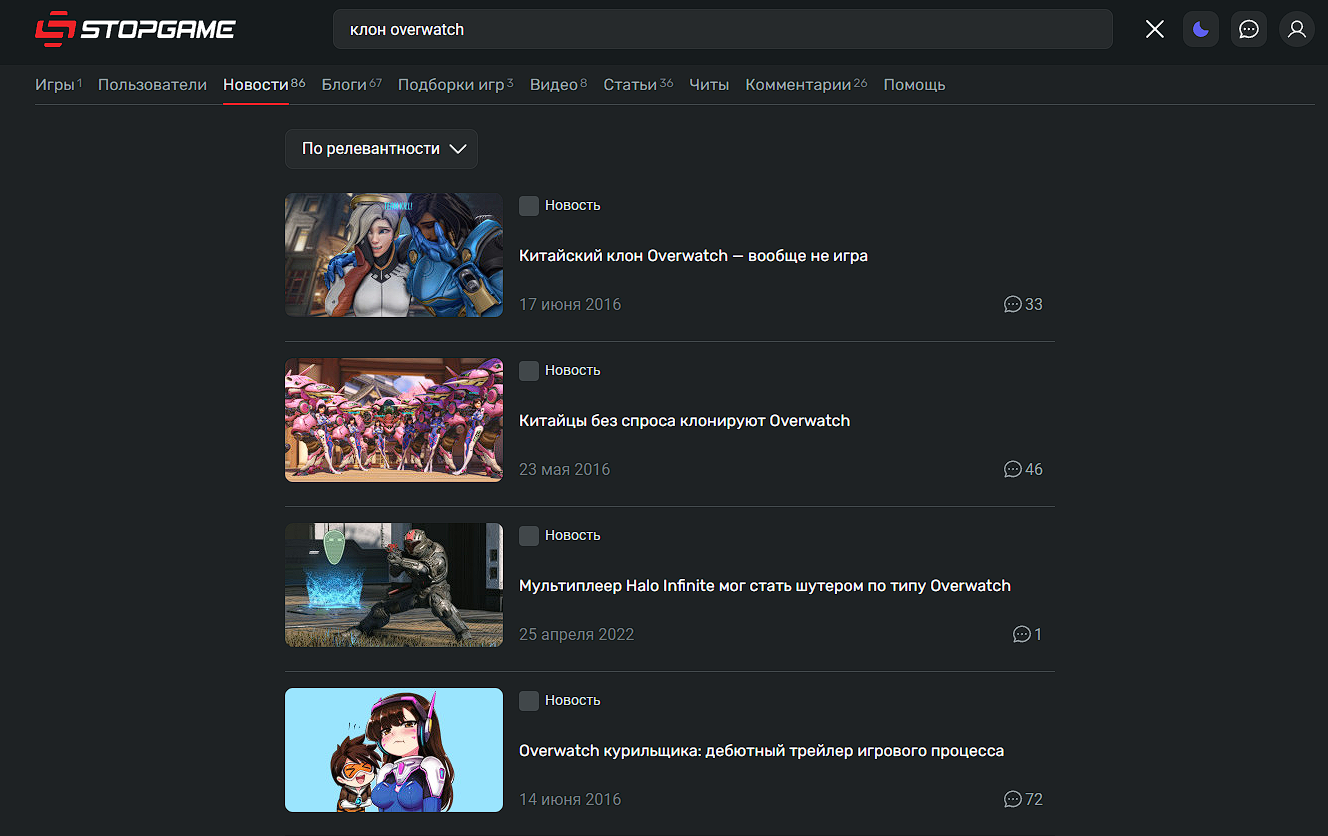
\includegraphics[width=\textwidth, height=\textheight, keepaspectratio]{pics/stopgame_search.png}

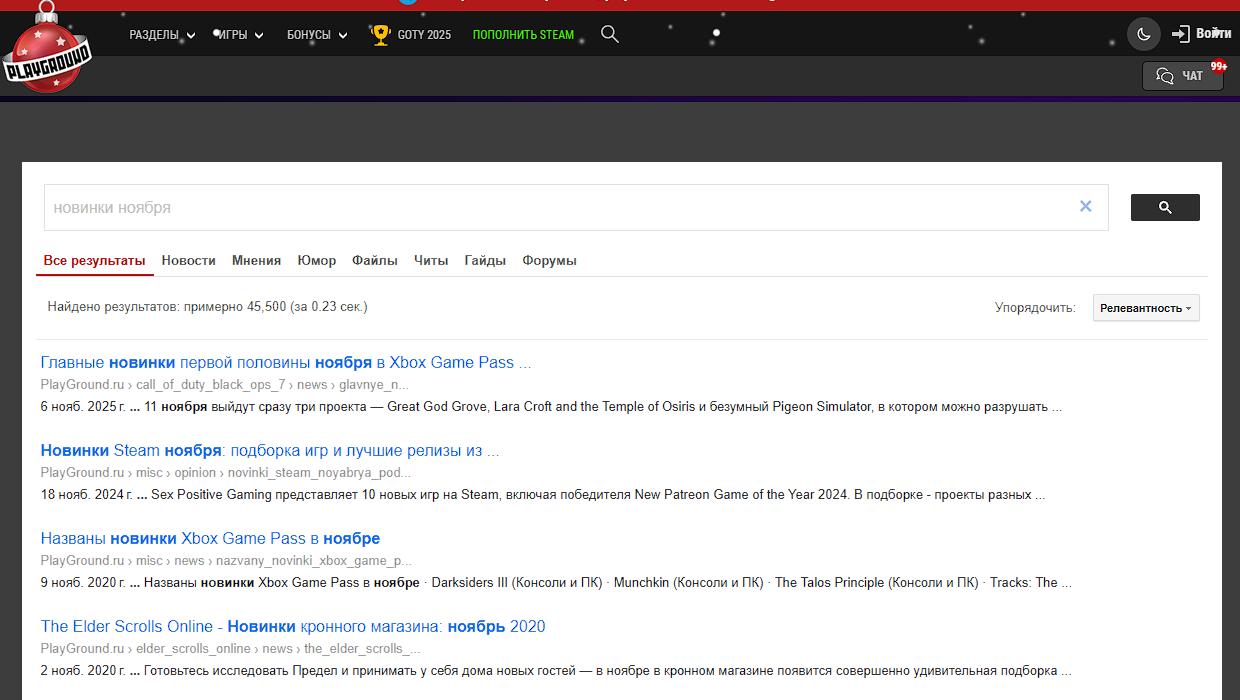
\includegraphics[width=\textwidth, height=\textheight, keepaspectratio]{pics/playground_search.png}

\vspace{1 em}
\noindent\textbf{Характеристики и разметка текста.} html-структура документов включает:
\begin{itemize}
    \item В разделе \texttt{<head>} присутствуют теги \texttt{<title>}, \texttt{<meta name="description">}, \texttt{<meta name="keywords">}, а также разметка Open Graph (\texttt{og:}) и Schema.org для улучшения отображения в социальных сетях и поисковых системах.
    \item Текст статьи или обзора размещен внутри тегов \texttt{<body>}. Полезный контент окружен тегами (\texttt{<article>}, \texttt{<h1>}-\texttt{<h6>}, \texttt{<p>}), но присутствует большое количество разметки для навигации, рекламы, комментариев и сторонних скриптов.    
\end{itemize}

\vspace{1 em}
\noindent\textbf{Статистика корпуса.} Статистика была собрана с помощью Python-скрипта

\begin{table}[h]
\centering
\begin{tabular}{|l|r|l|}
\hline
Статистика & Значение & Единица \\
\hline
Число документов & 35274 & Шт \\
\hline
Общий размер сырых данных & 7116.87 & Мб \\
\hline
Общий размер текста & 368.44 & Мб \\
\hline
Средний размер документа & 0.20 & Мб \\
\hline
СРедний размер текста & 7.57 & Кб \\
\hline
\end{tabular}
\end{table}

Из сырых 7.12 Гб html-данных было извлечено лишь 368 Мб текста (примерно 5.05\% от общего объема), это типично для современных веб-документов, где основную массу составляют разметка, стили и скрипты. Средний размер извлеченного из статьи текста 7.57 Кб - это относительно короткие статьи, думаю, что это характерно для новостных и обзорных публикаций на игровых порталах.



\pagebreak

